\chapter{Criterios de optimización y ordenamiento para conjuntos ordenados}

En este capítulo se describen en detalle los diferentes \textbf{criterios de optimización}, así como los \textbf{criterios de ordenamiento} empleados en las operaciones para conjuntos ordenados. Ambos conjuntos de criterios se aplicarán posteriormente con el objetivo de mejorar la eficiencia general de las operaciones y reducir significativamente los tiempos de ejecución.

Ahora bien, para que todo este claro, un criterio de optimización es en esencia un predicado que permite deduci

\textbf{Pseudocódigo y notación:} En este capítulo, al igual que se hizo para los conjuntos desordenados, se emplearán subíndices para referirse a los multi-intervalos de un conjunto ordenado. Dado un conjunto ordenado $A$, el elemento ubicado en la posición $i$, lo cual corresponde a \texttt{pieces\_[i]} en C++, se denotará como \textbf{$A_i$}, donde $i$ es un número natural que satisface $0 \leq i < |A|$, siendo $|A|$ el cardinal del conjunto $A$, es decir, la cantidad total de elementos que contiene. Cabe destacar que, al tratarse de un conjunto ordenado, siempre se cumple que $A_i < A_j$ si y sólo si $i < j$, para todo par de $i$ y $j$ tal que $0  \leq i, j < |A|$. Adicionalmente se dirá que, en el caso anterior $A_i$ esta \textbf{antes} de $A_j$ en $A$, mientras $A_j$ esta \textbf{después} de $A_i$

\section{Intersección - \texttt{intersection}}

La operación \texttt{intersection} constituye un componente central dentro de la batería de operaciones fundamentales para conjuntos. Antes de presentar las optimizaciones específicas y su correspondiente criterio de ordenamiento, es conveniente recordar el funcionamiento general de la intersección de conjuntos:

\begin{center}
\textit{Para intersecar dos conjuntos se debe considerar que cada conjunto está compuesto por multi-intervalos. Por lo tanto, la operación consiste en evaluar todas las posibles intersecciones de los multi-intervalos de uno de los conjunto con los del otro conjunto participante .}
\end{center}

Esto se puede ver en el pseudocódigo de la operación \texttt{intersección} para conjuntos desordenados ~\ref{alg:interseccionDes}.
\subsection{Criterios de optimización}

\subsubsection{Criterio de parada}

\begin{center}
    \textit{Supongase que se lleva a cabo la intersección entre $A$ y $B$, dos conjuntos ordenados, y se están considerando las posibles intersecciones del multi-intervalo \( i \)-ésimo de $A$, \( A_i \), con todos los multi-intervalos de $B$.}
\end{center}

\begin{figure}[h]
     \centering
    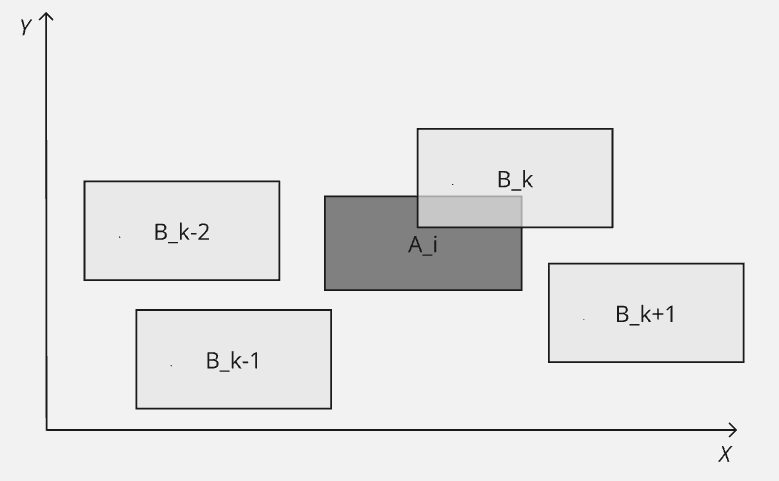
\includegraphics[width=0.75\linewidth]{figures/Optimazaciones/Interseccion/interseccion1a1.png}\par
    \caption{Ejemplificación de una iteración del proceso de intersección sobre dos conjuntos A y B.}
    \label{fig:enter-label}
\end{figure}

En algún punto, puede que se alcance un valor $k$, con $0 \leq k < |B|$, tal que el elemento mínimo de $B_k$ sea estrictamente mayor, en su primera dimensión (dimensión $x$ o $0$), que el elemento máximo de $A_i$. Por ejemplo, si el mínimo de $B_k$ es $(3,5)$ y el máximo de $A_i$ es  $(2,3)$. En este caso, se pueden derivar las siguientes conclusiones:

\begin{itemize}
     \item La intersección entre $A_i$ y $B_k$ resulta vacía, ya que como todos los valores de $A_i$ tienen un valor menor o igual que el máximo de $A_i$ en la primera dimensión, todos los valores de $B_k$ tienen un valor mayor o igual que el mínimo de $B_k$ en la primera dimensión y, como se vio, el elemento mínimo de $B_k$ sea estrictamente mayor en su primera dimensión que el elemento máximo de $A_i$, entonces ningún elemento de $A_i$ esta en $B_k$
    
    \item Debido al orden creciente de los conjuntos por el operador $<$ de multi-intervalos, cualquier multi-intervalo $B_{k'}$ con $k < k' < |B|$ tendrá en la primera dimensión de su mínimo un valor mayor o igual que el mínimo de $B_k$ en dicha dimensión, lo cual garantiza que también será vacía su intersección con $A_i$.
\end{itemize}

\begin{figure}[h]
    \centering
    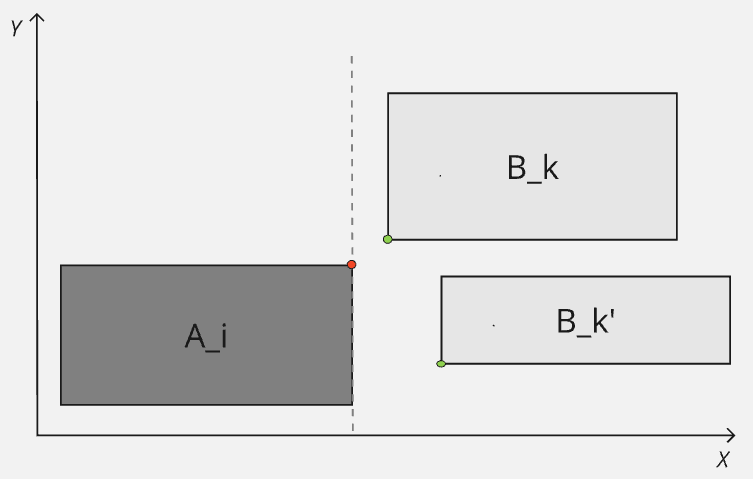
\includegraphics[width=0.75\linewidth]{figures/Optimazaciones/Interseccion/criterio de parada.png}
    \caption{Criterio de parada.}
    \label{fig:criterio-parada}
\end{figure}

En consecuencia, se puede establecer el siguiente criterio fundamental para optimizar la intersección entre conjuntos ordenados:

\begin{center}
    \fbox{
        \parbox{0.92\linewidth}{
            \centering
            \textbf{Criterio de parada} \\[1ex]
            \raggedright
            Sean $A$ y $B$ dos conjuntos ordenados. Supóngase que se está evaluando la intersección entre ambos, y en particular se consideran las posibles intersecciones entre un multi-intervalo $A_i$ de $A$, con $0 \leq i < |A|$, y los multi-intervalos de $B$. Dado un índice $k$ tal que $0 \leq k < |B|$, vale lo siguiente:

            \vspace{0,5cm}
     
            \textbf{Si} el máximo de $A_i$ es estrictamente menor que el mínimo de $B_k$ en la primera dimensión, \textbf{entonces}:

            \begin{itemize}
                \item la intersección entre $A_i$ y $B_{k'}$ resulta vacía, $\forall k' \mid k \leq k' < |B|$,
                \item \textbf{y, entonces} puede continuarse directamente con la evaluación de las intersecciones entre $A_{i+1}$(si existe) y los elementos de $B$ al no aceptar los conjuntos multi-intervalos vacíos.
            \end{itemize}
    
        }
    }
\end{center}

\subsubsection{Criterio de eliminación}

\begin{center}
    \textit{Nuevamente, supongase que se lleva a cabo la intersección entre $A$ y $B$, dos conjuntos ordenados, y se están considerando las posibles intersecciones del multi-intervalo \( i \)-ésimo de $A$, \( A_i \), con todos los multi-intervalos de $B$.}
\end{center}

En algún punto, puede que se alcance un valor $k$, con $0 \leq k < |B|$, tal que el elemento máximo de $B_k$ sea estrictamente menor, en su primera dimensión (dimensión $x$ o $0$), que el elemento mínimo de $A_i$. Por ejemplo, si el mínimo de $A_i$ es $(3,5)$ y el máximo de $B_k$ es  $(2,3)$. En este caso, se pueden derivar las siguientes conclusiones:

\begin{itemize}
     \item La intersección entre $A_i$ y $B_k$ resulta vacía, ya que como todos los valores de $A_i$ tienen un valor mayor o igual que el mínimo de $A_i$ en la primera dimensión, todos los valores de $B_k$ tienen un valor menor o igual que el máximo de $B_k$ en la primera dimensión y, como se vio, el elemento máximo de $B_k$ sea estrictamente menor en su primera dimensión que el elemento mínimo de $A_i$, entonces ningún elemento de $A_i$ esta en $B_k$

    \item Debido al orden creciente de los conjuntos por el operador $<$ de multi-intervalos, cualquier multi-intervalo $A_{i'}$ con $i < i' < |A|$ tendrá en la primera dimensión de su mínimo un valor mayor o igual que el mínimo de $A_i$ en dicha dimensión, lo cual garantiza que también será vacía su intersección con $B_k$.
\end{itemize}

\begin{figure}[h]
    \centering
    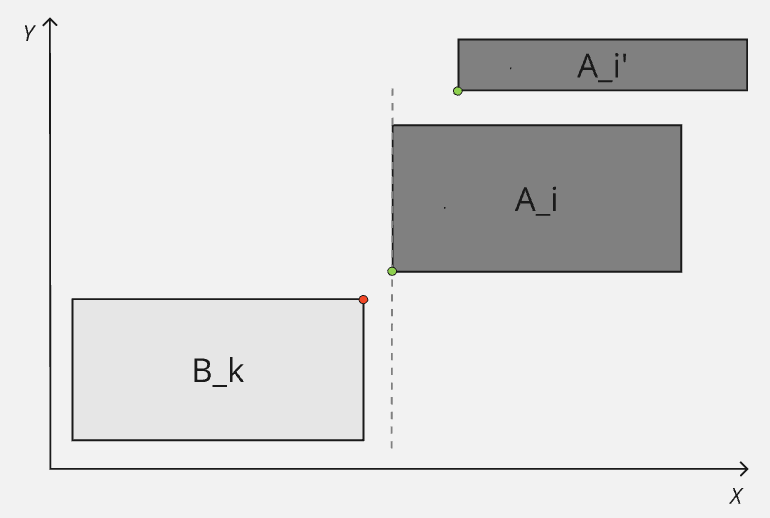
\includegraphics[width=0.75\linewidth]{figures/Optimazaciones/Interseccion/criterio de elim.png}
    \caption{Criterio de eliminación.}
    \label{fig:criterio-eliminacion}
\end{figure}

En consecuencia, se puede establecer el siguiente criterio fundamental para optimizar la intersección entre conjuntos ordenados:


\begin{center}
    \fbox{
        \parbox{0.92\linewidth}{
            \centering
            \textbf{Criterio de eliminación} \\[1ex]
            \raggedright
            Sean $A$ y $B$ dos conjuntos ordenados. Supóngase que se está evaluando la intersección entre ambos, y en particular se consideran las posibles intersecciones entre un multi-intervalo $A_i$ de $A$, con $0 \leq i < |A|$, y los multi-intervalos de $B$. Dado un índice $k$ tal que $0 \leq k < |B|$, vale lo siguiente:

            \vspace{0,5cm}
     
            \textbf{Si} el máximo de $B_k$ es estrictamente menor que el mínimo de $A_i$ en la primera dimensión, \textbf{entonces}:

            \begin{itemize}
                \item la intersección entre $A_{i'}$ y $B_{k}$ resulta vacía, $\forall i' \mid i \leq i' < |A|$,
                
                \item \textbf{y, entonces} puede descartarse $B_k$ para los cálculos de las posibles intersecciones de los multi-intervalos posteriores a $A_i$ al no aceptar los conjuntos multi-intervalos vacíos.
            \end{itemize}
    
        }
    }
\end{center}

Cabe señalar que, tanto para este criterio como para el anterior, no se especifica el tipo de multi-intervalo (si es denso o no), ya que dicha característica no afecta directamente la validez de los mismos.


\subsubsection{Criterio de selección}

Como se analizó en el criterio de eliminación, el procedimiento de intersección considera cada multi-intervalo del conjunto $A$ e intenta intersectarlo con todos los multi-intervalos del conjunto $B$. Y donde la idea central del criterio es que, a medida que se avanza en este proceso, ciertos elementos de $B$ pueden ser descartados progresivamente si se determina que ya no podrán intersectar con los siguientes elementos de $A$.

Naturalmente, se puede llegar al punto en el cual todos los elementos de $B$ habrán sido descartados, lo que implica que la operación \texttt{intersection} podrá finalizar directamente ya que no quedan intersecciones posibles a verificar.

Ahora bien, existe una observación importante respecto al tamaño de $B$: cuanto menor sea la cantidad de multi-intervalos en $B$, más rápido podrán descartarse todos ellos posiblemente, y por tanto, terminar la operación.

En base a esta idea, se introduce el \textbf{criterio de selección}, el cual establece lo siguiente:

\begin{center}
    \fbox{
        \parbox{0.9\linewidth}{
            \centering
            \textbf{Criterio de selección} \\[1ex]
            \raggedright
            Sean dos conjuntos ordenados involucrados en la operación de intersección. Se establece lo siguiente:

            \begin{center}
            \textit{
                Se define como $B$ a aquel conjunto que contiene la menor cantidad de multi-intervalos,
                mientras que se denota como $A$ al conjunto restante.
            }
            \end{center}
        }
    }
\end{center}

\subsubsection{Criterio de solapamiento}


Se introduce ahora el \textbf{criterio de solapamiento}, el cual establece lo siguiente:

\begin{center}
    \fbox{
        \parbox{0.93\linewidth}{
            \centering
            \textbf{Criterio de solapamiento} \\[1ex]
            \raggedright
            Sean $A$ y $B$ dos conjuntos, $A_i$ un multi-intervalo del conjunto $A$ y $B_k$ un multi-intervalo del conjunto $B$, con índices tales que:
            \[
            0 \leq i < |A|, \quad 0 \leq k < |B|.
            \]
            Se establece entonces que, en el caso de realizar la intersección entre $A$ y $B$:

            \begin{itemize}
                \item \textbf{Si} existe solapamiento entre $A_i$ y $B_k$, \textbf{entonces}:
                \begin{itemize}
                    \item \textbf{Si} ambos multi-intervalos son \textit{densos}, la intersección entre ellos es necesariamente no vacía y debe proceder.
                    \item \textbf{Si} al menos uno de ellos no es denso, la intersección \textit{puede} ser no vacía, pero no se garantiza de modo que se debe proceder de igual manera.
                \end{itemize}

                \item \textbf{Si} \textbf{no} existe solapamiento entre $A_i$ y $B_k$, \textbf{entonces} la intersección entre ellos es necesariamente vacía, independientemente de si son densos o no, y por ende puede obviarse su calculo.
            \end{itemize}
        }
    }
\end{center}

Ahora bien, seguiría explicar que es el solapamiento en si:

\begin{center}
    \textit{Sean dos multi-intervalos $m_1$ y $m_2$. Los multi-intervalos $m_1$ y $m_2$ se \textbf{solapan} \textbf{si}, \textbf{y sólo si}, todos sus intervalos componentes en cada dimensión se solapan.}

    \textit{Sean $a = [a_{\text{begin}} : a_{\text{step}} : a_{\text{end}}]$ y $b = [b_{\text{begin}} : b_{\text{step}} : b_{\text{end}}]$ dos intervalos. Se dice que se \textbf{solapan} \textbf{si}, \textbf{y sólo si}, se cumple alguna de las siguientes condiciones:}

$\neg (b_{\text{end}} < a_{\text{begin}} \lor a_{\text{end}} < b_{\text{begin}})$
\end{center}

Para ejemplificar mejor la noción de solapamiento en intervalos se proponen los siguientes casos en base a la predicado presentado por la definición:

\begin{itemize}
    \item \textbf{Primer caso:} Se cumple que $b_{\text{end}} < a_{\text{begin}}$ y $a_{\text{end}} < b_{\text{begin}}$ no.

    En este caso, no hay solapamiento. Por ejemplo, si $b = [1:1:5]$ y $a = [6:2:10]$, entonces $5 < 6$, por lo tanto, no se solapan.

    \begin{figure}[h]
        \centering
        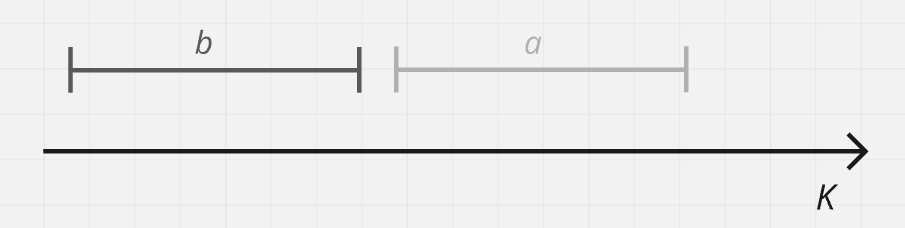
\includegraphics[width=0.75\linewidth]{figures/Optimazaciones/Interseccion/crit sol 10.png}
        \caption{Solapamiento sobre intervalos: \textit{primera condición verdadera}.}
    \end{figure}

    \item \textbf{Segundo caso:} No se cumple que $b_{\text{end}} < a_{\text{begin}}$ pero $a_{\text{end}} < b_{\text{begin}}$ si.

    Nuevamente, no hay solapamiento. Por ejemplo, si $b = [8:2:10]$ y $a = [4:2:6]$, entonces $6 < 8$.

    \begin{figure}[h]
        \centering
        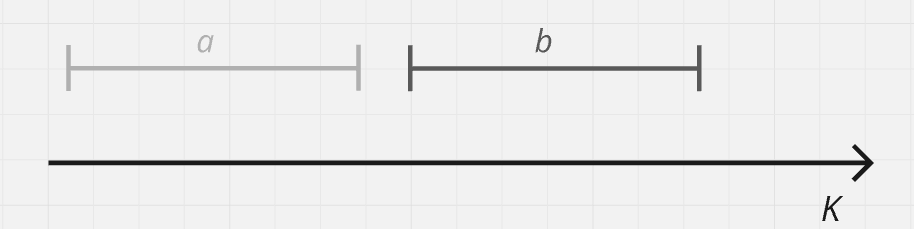
\includegraphics[width=0.75\linewidth]{figures/Optimazaciones/Interseccion/crit sol01.png}
        \caption{Solapamiento sobre intervalos: \textit{segunda condición verdadera}.}
    \end{figure}

    \item \textbf{Tercer caso:} Ninguna de las dos condiciones se cumple.

    En este caso resulta que se pueden dar dos situaciones unicamente: $b_{begin}$ o $b_{end}$ se encuentran entre $a_{begin}$ y $a_{end}$ inclusive(Figura~\ref{fig:crit-solapamiento-b}, Figura~\ref{fig:crit-solapamiento-c} y Figura~\ref{fig:crit-solapamiento-d}), ó $b_{begin} < a_{begin}$ y $b_{end}>a_{end}$(Figura~\ref{fig:crit-solapamiento-a}).

\begin{figure}[H]
    \centering

    \begin{subfigure}{0.75\linewidth}
        \centering
        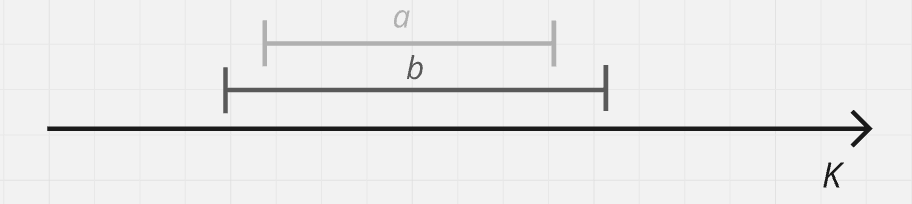
\includegraphics[width=\linewidth]{figures/Optimazaciones/Interseccion/crit sol 11 1.png}
        \caption{}
        \label{fig:crit-solapamiento-a}
    \end{subfigure}
    
    \vspace{0.4cm}

    \begin{subfigure}{0.75\linewidth}
        \centering
        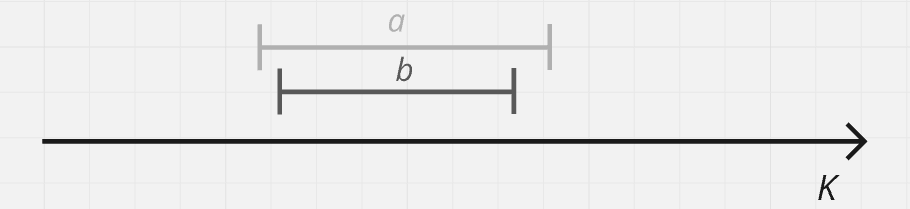
\includegraphics[width=\linewidth]{figures/Optimazaciones/Interseccion/crit sol 11 2.png}
        \caption{}
        \label{fig:crit-solapamiento-b}
    \end{subfigure}
    
    \vspace{0.4cm}

    \begin{subfigure}{0.75\linewidth}
        \centering
        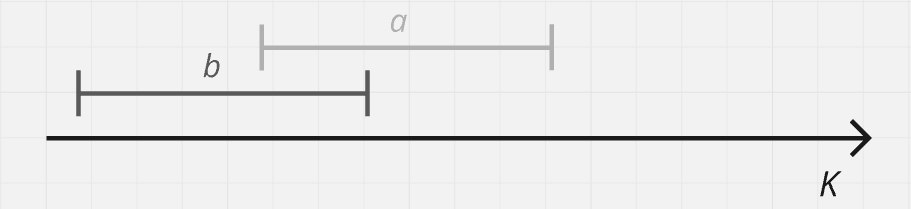
\includegraphics[width=\linewidth]{figures/Optimazaciones/Interseccion/crit sol 11 3.png}
        \caption{}
        \label{fig:crit-solapamiento-c}
    \end{subfigure}
    
    \vspace{0.4cm}

    \begin{subfigure}{0.75\linewidth}
        \centering
        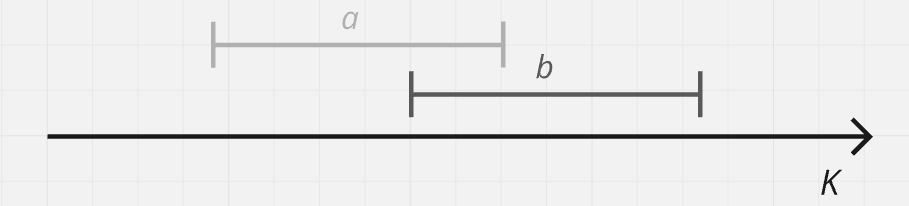
\includegraphics[width=\linewidth]{figures/Optimazaciones/Interseccion/crit sol 11 4.png}
        \caption{}
        \label{fig:crit-solapamiento-d}
    \end{subfigure}

    \caption{Solapamiento sobre intervalos: \textit{el predicado entero es falso}.}
    \label{fig:crit-solapamiento}
\end{figure}
        \item \textbf{Cuarto caso:} Las dos condiciones se cumplen.
        
        Cabe destacar que el caso en el cual \textbf{ambas condiciones} sean verdaderas simultáneamente es imposible. En efecto, si se cumple que:

        \[
        b_{\text{end}} < a_{\text{begin}} \quad \text{y} \quad a_{\text{end}} < b_{\text{begin}},
        \]
        
        entonces, por $a_{\text{begin}} < a_{\text{end}}$ y transitividad de la desigualdad, se deduce que:
        
        \[
        b_{\text{end}} < b_{\text{begin}},
        \]
        
        lo cual implicaría que el intervalo $b$ está mal definido, ya que su extremo final es menor que su extremo inicial. Esto contradice la definición válida de intervalo, por lo tanto, dicho caso \textbf{no} puede ocurrir.
\end{itemize}


Por un lado, se puede observar que si, en al menos una dimensión, los intervalos correspondientes de dos multi-intervalos $m$ y $p$, ya sean densos o no, no se solapan, entonces no existe ninguna $n$-upla $(m_0, \dots, m_{n-1}) \in m$ y $(p_0, \dots, p_{n-1}) \in p$ tal que coincidan en esa dimensión, con $n$ siendo la aridad de $m$ y $p$. En consecuencia, esto implica que la intersección entre $m$ y $p$ será vacía, independientemente de que en las demás dimensiones sí exista solapamiento.

Por otro lado, si en todas las dimensiones los intervalos correspondientes se solapan y ambos multi-intervalos son densos, entonces se garantiza la existencia de al menos una $n$-upla $(m_0, \dots, m_{n-1})$ perteneciente tanto a $m$ como a $p$. En efecto, basta con elegir un valor dentro del intervalo intersección para cada dimensión, lo cual es posible precisamente porque los intervalos son densos y contienen todos los valores posibles del $begin$ al $end$.

Sin embargo, si uno o ambos multi-intervalos no son densos, esta garantía desaparece. Aunque exista solapamiento en todas las dimensiones, podría no haber ninguna $n$-upla común, ya que en alguna dimensión podría ocurrir que, debido al paso distinto de 1, el intervalo solapamiento puede no tener valores a partir de los cuales elegir. Por ejemplo, en una dimensión se pueden contar con los intervalos $[5:5:10]$ y $[6:1:9]$, los cuales se solapan pero cuyo intervalo intersección es vació. 

\subsection{Criterio de ordenamiento}

Uno de los aspectos fundamentales a considerar al implementar la operación de intersección entre conjuntos ordenados es cómo construir el conjunto resultado de manera que conserve su orden intrínseco. En este contexto, el desafío consiste en insertar las intersecciones de los multi-intervalos en el conjunto resultado de la forma más eficiente posible, garantizando siempre que se mantenga la invariante del orden.

\begin{center}
    \fbox{
        \parbox{0.93\linewidth}{
            \centering
            \textbf{Criterio de ordenamiento} \\[1ex]
            \raggedright
            Supóngase que se realiza la intersección entre dos conjuntos ordenados, $A$ y $B$, y que se están evaluando las posibles intersecciones del $i$-ésimo multi-intervalo de $A$, denotado por $A_i$, con todos los multi-intervalos de $B$. Ademas se cuenta con un conjunto resultado $C$.

            \vspace{1ex}

            Todas las intersecciones no vacías generadas con $A_i$ deben insertarse en $C$ \textbf{después} de aquellas intersecciones generadas por los multi-intervalos $A_0, A_1, \dots, A_{i-1}$, cuyos mínimos sean estrictamente menores al de $A_i$, bajo el operador $<$ de naturales multi-dimensionales.
        }
    }
\end{center}


Este criterio se fundamenta en la observación de que la intersección entre dos multi-intervalos está contenida en ambos. Esto implica que el elemento mínimo de la intersección debe ser, necesariamente, un valor que pertenezca a ambos operandos, y por lo tanto debe coincidir con el mínimo de alguno de ellos, o bien ser un valor contenido en ambos.

Al fijar el multi-intervalo $A_i$ como decreta el criterio, se observa que cualquier intersección no vacía con un multi-intervalo $B_k$ del conjunto $B$ tendrá su mínimo dentro de $A_i$, o coincidirá con el mínimo de este. Como resultado, cualquier intersección no vacía generada tendrá un mínimo mayor, bajo el operador $<$ de naturales multi-dimensionales, o igual que el mínimo de $A_i$.

Esto garantiza que tales intersecciones deben insertarse en el conjunto resultado después de aquellas cuyo mínimo sea estrictamente menor, bajo el operador $<$ de naturales multi-dimensionales, al de $A_i$. 

La Figura~\ref{fig:enter-label} ilustra gráficamente esta situación. Como se observa, todas las intersecciones producidas a partir de $A_i$ tienen un mínimo mayor o igual que el de $A_i$, y se insertan a continuación de las intersecciones previamente procesadas cuyo mínimo sea menor al de $A_i$. Esto mismo ocurre con las de $A_{i+1}$

\begin{figure}[h]
    \centering
    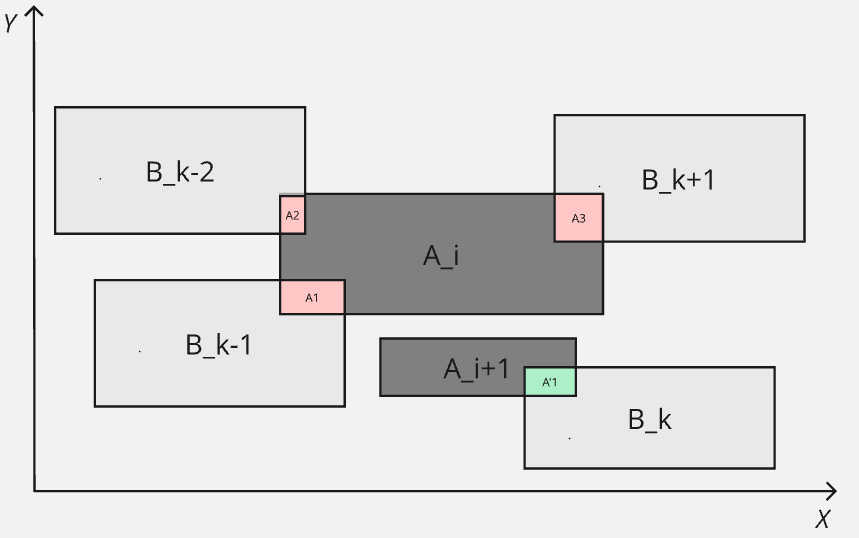
\includegraphics[width=0.7\linewidth]{figures/Optimazaciones/Interseccion/crit ordenamiento.png}
    \caption{Criterio de ordenamiento en la intersección de conjuntos ordenados.}
    \label{fig:enter-label}
\end{figure}

Adicionalmente, no es necesario comenzar a verificar la posición de inserción de las intersecciones en el conjunto resultado desde el principio en cada iteración de los elementos de $A$. Dado el orden intrínseco de los conjuntos involucrados, se cumple que:
\begin{center}
    \textit{El mínimo de $A_i$ es menor, bajo el operador $<$ de naturales multi-dimensionales, al mínimo de $A_{i+1}$}
\end{center}

Esto implica, en conjunto con lo establecido previamente sobre los mínimos de las intersecciones generadas, que todas las intersecciones obtenidas a partir de $A_{i+1}$ con los elementos de $B$ deben insertarse en el conjunto resultado a partir de una posición \textbf{igual o posterior} a aquella en la que comenzaron a insertarse las intersecciones de $A_i$ con $B$.

Por lo tanto, el criterio de ordenamiento puede refinarse del siguiente modo:



\begin{center}
    \fbox{
        \parbox{0.93\linewidth}{
            \centering
            \textbf{Criterio de ordenamiento} \\[1ex]
            \raggedright
            Supóngase que se realiza la intersección entre dos conjuntos ordenados, $A$ y $B$, y que se están evaluando las posibles intersecciones del $i$-ésimo multi-intervalo de $A$, denotado por $A_i$, con todos los multi-intervalos de $B$. Ademas se cuenta con un conjunto resultado $C$.

            \vspace{1ex}

            Todas las intersecciones no vacías generadas con $A_i$ deben insertarse en $C$ \textbf{después} de aquellas intersecciones generadas por los multi-intervalos $A_0, A_1, \dots, A_{i-1}$, cuyos mínimos sean estrictamente menores al de $A_i$, bajo el operador $<$ de naturales multi-dimensionales.
            
            \vspace{1ex}

            Adicionalmente \textbf{si} la posición a partir de la cual se colocan las intersecciones de $A_i$ en el conjunto resultante es $k$, con $0 \leq k < |C|$, \textbf{entonces} aquellas generadas por $A_{i+1}$ se insertaran a partir de $k'$ tal que $k \leq k' < |C|$.
        }
    }
\end{center}



Esta optimización reduce significativamente la cantidad de comparaciones necesarias para ubicar cada intersección, manteniendo la eficiencia del proceso y evitando retrocesos innecesarios dentro de la estructura del conjunto ordenado resultante.


\section{Unión disjunta - \texttt{disjointCup}}

La operación \texttt{disjointCup} se encarga de realizar la unión disjunta entre dos conjuntos de multi-intervalos que, por hipótesis, son disjuntos. En particular, esta operación simplemente coloca los elementos de ambos conjuntos en uno solo, sin aplicar ningún tipo de transformación adicional ni sobre los argumentos ni sobre el contenido de sus elementos. Esto se puede ver muy bien particularmente en el pseudocódigo de esta para conjuntos desordenados \ref{alg:disjointcupDes}.

Ahora bien, al trabajar con conjuntos \textit{ordenados}, resulta necesario introducir un criterio de ordenamiento que garantice que el conjunto resultante mantenga el orden. Este criterio de ordenamiento se presenta a continuación.

\subsection{Criterio de ordenamiento}

Dado que la función \texttt{disjointCup} se encarga de realizar la fusión de dos conjuntos ordenados en esta ocasión, es fundamental establecer con claridad el \textbf{criterio de ordenamiento}.

\begin{center}
    \fbox{
        \parbox{0.93\linewidth}{
            \centering
            \textbf{Criterio de ordenamiento}\\[1ex]
            \raggedright
            Sean $A = \{A_0, A_1, \dots, A_{n-1}\}$ y $B = \{B_0, B_1, \dots, B_{m-1}\}$ dos conjuntos no vacíos de multi-intervalos, disjuntos y ordenados. Sea $C$ un conjunto ordenado que contendrá el resultado de la fusión de $A$ y $B$. Y sean $A_i$ un multi-intervalo del conjunto $A$ y $B_k$ un multi-intervalo del conjunto $B$, con índices tales que:
            \[
            0 \leq i < |A|, \quad 0 \leq k < |B|.
            \]
            
            \vspace{1ex}

            Entonces, al realizar la unión disjunta entre $A$ y $B$ vale que:

            \begin{itemize}
                \item \textbf{Si $A_i < B_k$}, entonces $A_i$ debe insertarse en $C$ \textbf{antes} que $B_k$.
                \item \textbf{Si $B_k < A_i$}, entonces $B_k$ debe insertarse en $C$ \textbf{antes} que $A_i$.
            \end{itemize}

            \vspace{1ex}
        }
    }
\end{center}

Como se puede ver, el criterio unicamente se basa en el orden intrínseco de los conjuntos y no es para nada complejo o enrevesado.

\section{Complemento - \texttt{complement / complementAtom}}

Esta sección se dividirá en dos partes, ya que la operación de complemento para conjuntos ordenados, al igual que su contraparte de conjuntos desordenados, se compone de dos etapas: el \textit{complemento atómico} (\texttt{complementAtom}), que calcula el complemento de un conjunto ordenado representado por un único multi-intervalo; y el \textit{complemento general} (\texttt{complement}), la operación principal del complemento, que extiende esta operación tal que sea posible calcular el complemento de conjuntos ordenados compuestos por múltiples multi-intervalos a través de la operación \texttt{intersection}.

\subsection{Complemento atómico(\texttt{complementAtom})}

En el capítulo de conceptos previos se presentó el funcionamiento y la lógica de la construcción del conjunto complemento de un conjunto atómico, un conjunto compuesto por un único multi-intervalo, mediante la operación \texttt{complementAtom}, en el contexto de los conjuntos desordenados.

Tal como se mencionó, la estructura general de la implementación de las operaciones para conjuntos ordenados se basa en la utilizada para conjuntos desordenados. Por esta razón, correspondería ahora optimizar dicha operación teniendo en cuenta el orden y adaptarla para conjuntos ordenados.

Sin embargo, dado que el conjunto base contiene únicamente un multi-intervalo y solo contamos con un único conjunto como argumento de la operación, no hay margen para aplicar ninguna optimización basada en el orden de los argumentos de entrada. 

Por lo tanto, la única tarea pendiente es poder construir un conjunto ordenado resultado, lo cual implica determinar el \textbf{criterio de ordenamiento}.

\subsubsection{Criterio de ordenamiento}

En \texttt{complementAtom} se trabaja con dos tipos de multi-intervalos: \textit{all} y \textit{during}. Las transformaciones sucesivas de estos intervalos conforman el complemento del conjunto atómico. El uso de cada uno es el siguiente:

Sea $i$ un numero natural que hace referencia una dimensión entre $0$ y la cantidad de dimensiones del conjunto atómico procesado.
\begin{itemize}
  \item \textbf{\textit{all}}:  
    Construye el multi-intervalo ($\textit{all}_{i,b}$) que va desde $0$ hasta el inicio del multi-intervalo del conjunto en la dimensión $i$, siempre que exista.

  \item \textbf{\textit{during}} :  
    Cuando el multi-intervalo del conjunto no es denso en la dimensión $i$, es decir, el paso de la $i$-esima dimensión ($\text{paso}_i$) es distinto de $1$, se generan una serie de multi-intervalos intermedios ($\textit{during}_{i,c}$). Cada uno arranca en
    \[
      \bigl(\text{begin}_i\bigr) + c,
      \quad c = 1, 2, \dots, (\text{paso}_i - 1),
    \]
    donde $\text{begin}_i$ es el inicio en la dimensión $i$ del multi-intervalo del conjunto.

  \item \textbf{\textit{all}} :  
    Construye el multi-intervalo ($\textit{all}_{i,e}$) que va desde el final del multi-intervalo del conjunto en la dimensión $i$ hasta \texttt{Inf}, siempre que sea posible.
\end{itemize}

Sin embargo, al realizar el procesamiento secuencial de cada dimensión, es necesario tener en cuenta cómo los inicios de los intervalos correspondientes a las dimensiones ya recorridas del multi-intervalo  se propagan hacia $all$ y $during$. 

Una vez completados los cálculos en la dimensión $j$ (creación de \textit{all}$_{j,b}$, \textit{all}$_{j,e}$ y todos los \textit{during}$_{j,c}$), tanto \textit{during} como \textit{all} se modifican en dicha dimensión. A \textit{all} se le remplaza el intervalo en esa dimensión por el del multi-intervalo del conjunto en la misma dimensión pero con paso 1, y a \textit{during} se le hace lo mismo pero con el intervalo original.

Como consecuencia, todos los multi-intervalos que se generen en la siguiente dimensión $j+1$ tienen el mismo valor de inicio en la dimensión $j$ que tiene el multi-intervalo del conjunto. Por lo tanto los inicios de \textit{all}$_{i,b}$, \textit{all}$_{i,e}$ y de cada \textit{during}$_{i,c}$ coinciden, en las dimensiones $0,1,\ldots,i-1$, con los del multi-intervalo atómico original. Lo que conlleva a que el siguiente conjunto este ordenado:

\[
\{\textit{all}_{i,b},\;\textit{during}_{i,1},\;\textit{during}_{i,2},\;\dots,\;\textit{during}_{i,k},\;\textit{all}_{i,e}\}
\]

Pero ahora queda ver que interacción hay entre los conjuntos de cada dimensión para ver como ordenar la totalidad de los multi-intervalos de todas las dimensiones en un único conjunto.

Al estar en una dimensión $i$ y al haber terminado de generar los multi-intervalos de esa dimensión a través de \textit{during} y \textit{all}, por como son las modificaciones a estos dos multi-intervalos, resulta que todos los multi-intervalos generados en la dimensión $i+1$ van inmediatamente después de $all_{i,b}$(si existe), ya que en la dimensión $i$ tiene un valor de inicio $0$; y antes de los \textit{during}$_{i,c}$, cuyo inicio en la dimensión $i$ es el mismo que el de los multi-intervalos generados en $i+1$ pero mas una constante $c$. Como resultado tenemos que se da el siguiente orden:

\begin{align*}
\{ &\textit{all}_{x,b},\ \textit{all}_{y,b},\ \textit{all}_{z,b}, \\
   &\textit{during}_{z,1},\ \textit{during}_{z,2},\ \dots,\ \textit{during}_{z,k}, \\
   &\textit{all}_{z,e},\ \textit{during}_{y,1},\ \textit{during}_{y,2},\ \dots,\ \textit{during}_{y,j}, \\
   &\textit{all}_{y,e},\ \textit{during}_{x,1},\ \textit{during}_{x,2},\ \dots,\ \textit{during}_{x,j}, \\
   &\textit{all}_{x,e} \}
\end{align*}

trabajando con un conjunto atómico de tres dimensiones.

A partir de todo lo analizado previamente, se arriba a la siguiente formulación del criterio de ordenamiento para \texttt{complementAtom}:

\begin{center}
    \fbox{
        \parbox{0.93\linewidth}{
            \centering
            \textbf{Criterio de ordenamiento}\\[1ex]
            \raggedright
            El patrón general de inserción en las estructuras auxiliares $all$ y $during$, al recorrer las dimensiones en orden creciente, responde a la siguiente disposición:

            \begin{align*}
            \{ &\textit{all}_{0,b},\ \textit{all}_{1,b},\ \dots,\ \textit{all}_{d-1,b}, \\
               &\textit{during}_{d-1,1},\ \dots,\ \textit{during}_{d-1,k_{d-1}}, \\
               &\textit{all}_{d-1,e},\ \textit{during}_{d-2,1},\ \dots,\ \textit{during}_{d-2,k_{d-2}}, \\
               &\quad\vdots \\
               &\textit{all}_{1,e},\ \textit{during}_{0,1},\ \dots,\ \textit{during}_{0,k_0}, \\
               &\textit{all}_{0,e} \}
            \end{align*}

            \vspace{1ex}

            donde $d$ representa la aridad del conjunto (es decir, la cantidad de dimensiones), y $k_i$ indica la cantidad de pasos definidos en la dimensión $i$.
        }
    }
\end{center}



\subsection{Complemento general}

La operación \texttt{intersection} se utiliza como herramienta para calcular el complemento entre dos conjuntos desordenados en la operación \texttt{complement}: uno que representa el complemento de un conjunto de multi-intervalos desordenados, y otro que representa el complemento de un conjunto con un único multi-intervalo.

Teóricamente, podría utilizarse una única implementación general de \texttt{intersection}, como se hace en el caso de conjuntos desordenados y no modificar \texttt{complement} para el caso de conjuntos ordenados. Sin embargo, al tratarse de conjuntos ordenados, es posible aplicar ciertas optimizaciones adicionales, además de las ya detalladas en la sección correspondiente a \texttt{intersection}, que permiten mejorar el rendimiento de la operación. Es decir, se utilizara una versión adaptada de la intersección de conjuntos para el complemento.

\subsubsection{Intersección complementaria}

En esta modificación de la operación de intersección, denominada \texttt{intersectionComp}, se preservan los criterios de \textbf{parada}, \textbf{eliminación}, \textbf{solapamiento} y \textbf{ordenamiento}. Además de suponer que los conjuntos recibidos están ordenados, esta variante introduce una hipótesis adicional: los argumentos deben respetar un orden específico. El primer conjunto debe representar el complemento de un conjunto de multi-intervalos (posiblemente varios), mientras que el segundo conjunto corresponde al complemento de un único multi-intervalo. 

En otras palabras:
\begin{itemize}
    \item El primer conjunto, que denotara $A$, actúa como un \emph{complemento acumulado}.
    \item El segundo conjunto, denotado $B$, funciona como un \emph{complemento unitario}.
\end{itemize}

\textbf{Importante:} Para facilitar la siguiente explicación, se asume que los multi-intervalos involucrados son siempre densos.

Supongase ahora que el conjunto $A$ representa el complemento de un único multi-intervalo, al igual que $B$. Esta situación se ilustra en la Figura~\ref{fig:tra}.

\begin{figure}[htbp]
    \centering
    \begin{minipage}[t]{0.49\textwidth}
        \centering
        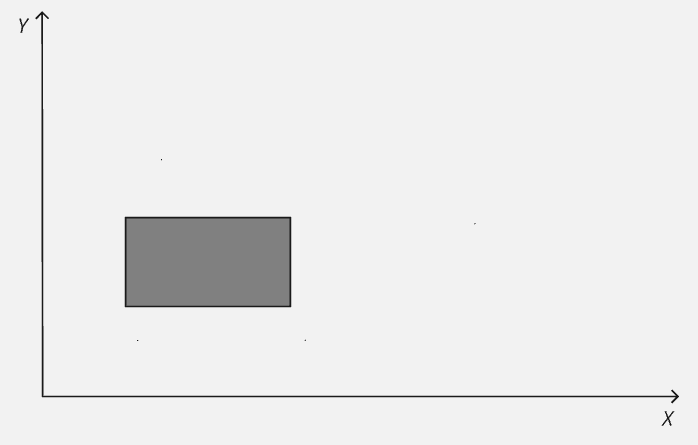
\includegraphics[width=\linewidth]{figures/Optimazaciones/Complement/Aelem.png}
        \caption*{\small Multi-intervalo generador de $A$}
        \vspace{8pt}
        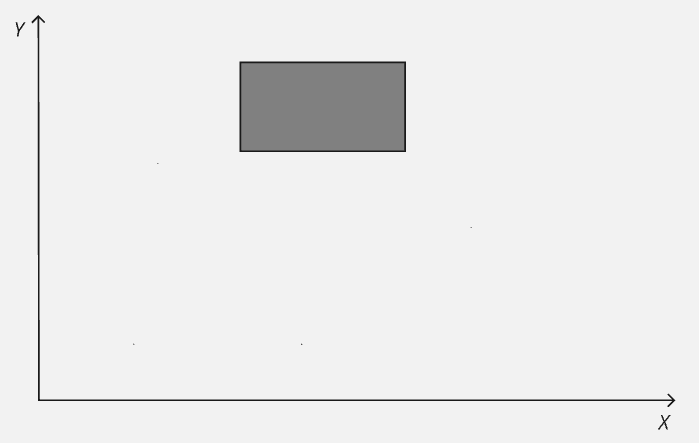
\includegraphics[width=\linewidth]{figures/Optimazaciones/Complement/Belem.png}
        \caption*{\small Multi-intervalo generador de $B$}
    \end{minipage}%
    \hspace{0.01\textwidth}
    \begin{minipage}[t]{0.49\textwidth}
        \centering
        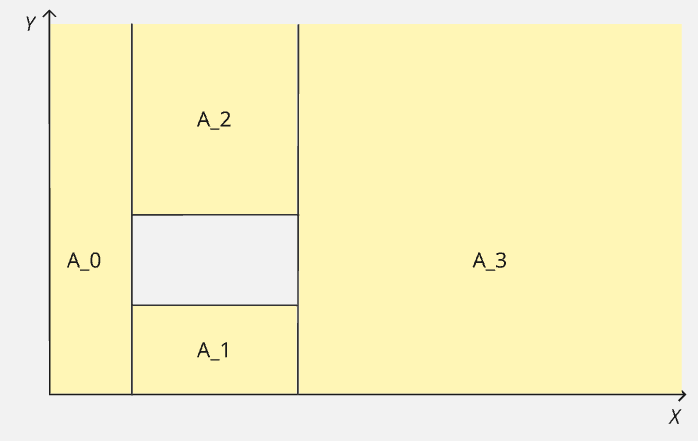
\includegraphics[width=\linewidth]{figures/Optimazaciones/Complement/A.png}
        \caption*{\small Conjunto complemento $A$}
        \vspace{8pt}
        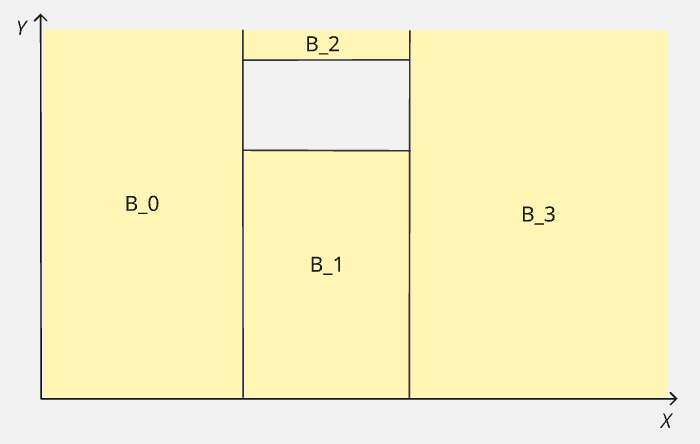
\includegraphics[width=\linewidth]{figures/Optimazaciones/Complement/B.png}
        \caption*{\small Conjunto complemento $B$}
    \end{minipage}
    \caption{Ejemplo gráfico de los conjuntos complemento de $A$ y $B$.}
    \label{fig:tra}
\end{figure}

Si se aplicara directamente la operación \texttt{intersection}, utilizando su versión optimizada para conjuntos ordenados, el resultado obtenido sería el ilustrado en la Figura~\ref{fig:compleAnt}. 

Sin embargo, puede observarse que se produce una partición adicional innecesaria: los multi-intervalos $C\_1$ y $C\_3$ podrían haberse mantenido como un único multi-intervalo. Esta fragmentación/particionamiento es consecuencia del funcionamiento de la operación intersección. No obstante, ambos multi-intervalos no comparten ningún elemento con el multi-intervalo generador de $B$, por lo que no deberían verse afectados ni sufrir ninguna sustracción de elementos al quitar de $A$ los elementos del multi-intervalo generador de $B$ a través de la intersección de $A$ y $B$.


\begin{figure}[htbp]
    \centering
    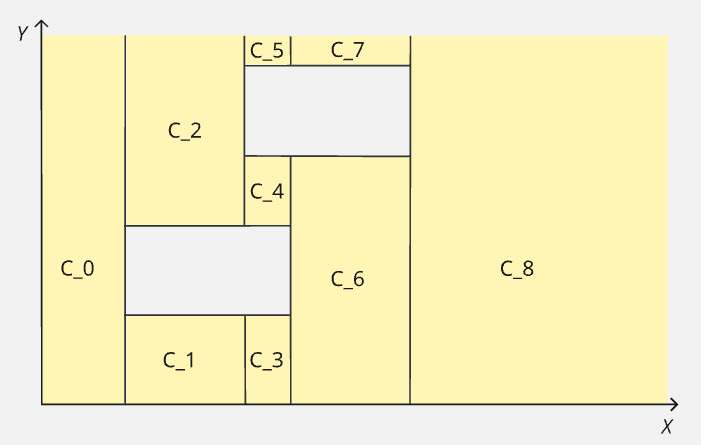
\includegraphics[width=0.8\linewidth]{figures/Optimazaciones/Complement/complAnt.png}
    \caption{Conjunto complemento resultante de la intersección entre $A$ y $B$, sin aplicar optimización.}
    \label{fig:compleAnt}
\end{figure}

Este tipo de fragmentación innecesaria puede evitarse mediante el \textbf{criterio de anti-particionamiento}, que establece lo siguiente:

\begin{center}
    \fbox{
        \parbox{0.93\linewidth}{
            \centering
            \textbf{Criterio de anti-particionamiento} \\[1ex]
            \raggedright
            Sea $A$ un conjunto complemento y $B$ el complemento de un conjunto compuesto por un único multi-intervalo $m$. Al realizar la intersección entre $A$ y $B$ durante el cálculo del complemento de un conjunto, se cumple que:
            
            \vspace{1ex}
            Todo multi-intervalo de $A$ que no se solape con el multi-intervalo $m$ generado por $B$ no requiere ser intersectado con los elementos de $B$, y debe copiarse directamente al conjunto resultado.
        }
    }
\end{center}


Aplicando este criterio, el conjunto complemento resultante se muestra en la Figura~\ref{fig:compleNue}, donde se observa una representación más compacta: se evita una partición innecesaria y se obtiene un conjunto más chico.

\begin{figure}[htbp]
    \centering
    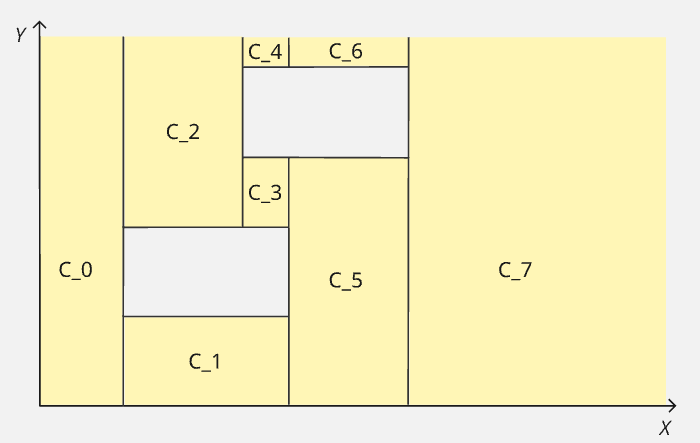
\includegraphics[width=0.8\linewidth]{figures/Optimazaciones/Complement/complNue.png}
    \caption{Conjunto complemento resultante tras aplicar el criterio de anti-particionamiento.}
    \label{fig:compleNue}
\end{figure}

Cabe destacar que este criterio también es válido cuando se trabaja con multi-intervalos no densos, y resulta especialmente útil en esos casos, ya que evita múltiples operaciones de posicionamiento y comparación innecesarias.

Si bien la reducción en el número de multi-intervalos resultantes puede parecer ínfima, es importante tener en cuenta que en la operación \texttt{complement} se aplica de forma acumulativa esta reducción. Por lo tanto, reducir la cantidad de particiones en cada iteración tiene un efecto significativo en el rendimiento total, ya que disminuye la cantidad de elementos a recorrer y comparar en las iteraciones posteriores.

Existe además una mejora adicional que puede aplicarse a la operación de intersección en el contexto del complemento. Esta surge del modo en que se construye el complemento ordenado de un conjunto atómico, tal como se explicó en la subsección correspondiente del complemento atómico.

En dicha construcción, el primer multi-intervalo del complemento ordenado es $\textit{all}_{x,b}$. Este multi-intervalo es denso y se extiende hasta el infinito en todas sus dimensiones, con excepción de la primera, donde finaliza una posición antes del comienzo del multi-intervalo original que dio lugar al complemento.

Adicionalmente se cumple que la intersección entre cualquier multi-intervalo y uno denso, que lo contiene por completo, es simplemente el multi-intervalo contenido. Es decir, si un multi-intervalo $m$ está completamente contenido en otro multi-intervalo denso $n$, entonces la intersección entre $m$ y $n$ es igual a $m$.

A partir de las observaciones anteriores, puede establecerse el \textbf{criterio de obviedad}, el cual permite evitar cálculos innecesarios durante la intersección del complemento, y estipula lo siguiente:

\begin{center}
    \fbox{
        \parbox{0.93\linewidth}{
            \centering
            \textbf{Criterio de obviedad} \\[1ex]
            \raggedright
            Sea $A$ un conjunto complemento y $B$ el complemento de un conjunto compuesto por un único multi-intervalo $m$. Al realizar la intersección entre $A$ y $B$ durante el cálculo del complemento de un conjunto, se cumple que:

            \vspace{0,5cm}
            
            Todo multi-intervalo del conjunto $A$ cuyo máximo sea estrictamente menor en la primera dimensión que el mínimo multi-intervalo generador de $B$, $m$, puede incorporarse directamente al conjunto resultado de la intersección, sin necesidad de ser intersectado con los elementos de $B$.
        }
    }
\end{center}


\begin{comment}
    

\begin{figure}[htbp]
    \centering
    \begin{minipage}[t]{0.49\textwidth}
        \centering
        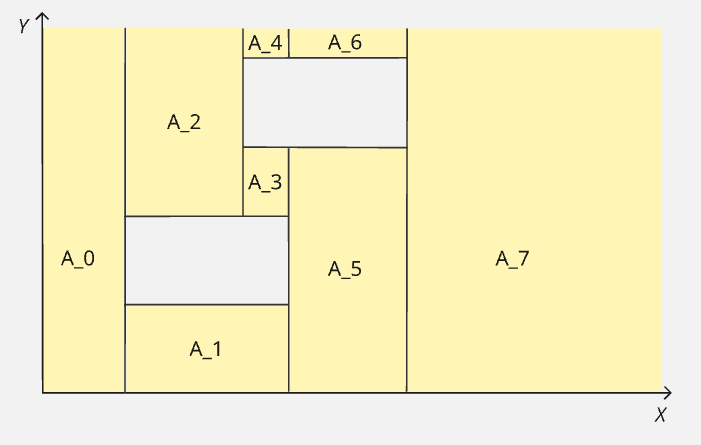
\includegraphics[width=\linewidth]{figures/Optimazaciones/Complement/Ao.png}
        \caption*{\small Conjunto complemento $A$}
    \end{minipage}%
    \hspace{0.01\textwidth}
    \begin{minipage}[t]{0.49\textwidth}
        \centering
        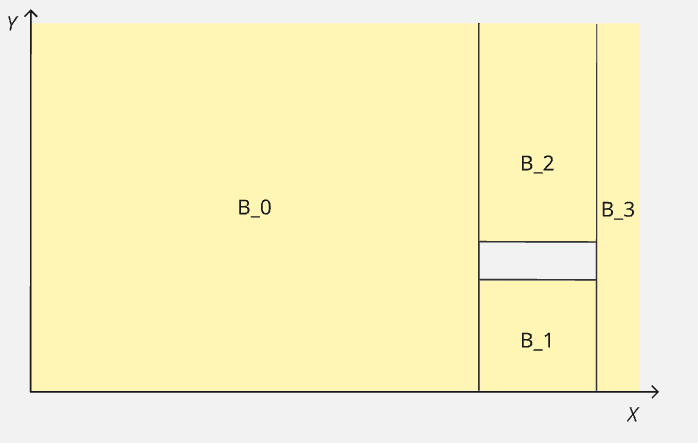
\includegraphics[width=\linewidth]{figures/Optimazaciones/Complement/Bo.png}
        \caption*{\small Conjunto complemento $B$}
    \end{minipage}
    \hspace{0.01\textwidth}
    \begin{minipage}[t]{0.49\textwidth}
        \centering
        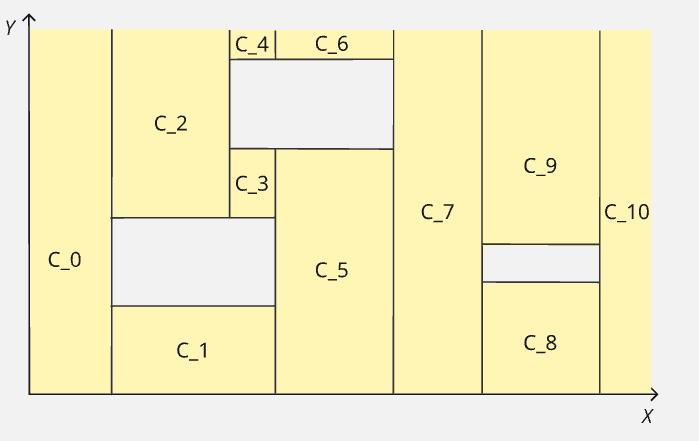
\includegraphics[width=\linewidth]{figures/Optimazaciones/Complement/complO.png}
        \caption*{\small Conjunto complemento resultante de la intersección}
    \end{minipage}
    \caption{Ejemplo gráfico de los conjuntos complemento $A$ y $B$.}
    \label{fig:tra}
\end{figure} 
\end{comment}


Tal como fue planteado, el \textbf{criterio de obviedad} permite evitar las comparaciones e intersecciones entre determinados multi-intervalos del conjunto complemento $A$ y los elementos del conjunto complemento $B$, pero su alcance inicial es limitado: únicamente evita el procesamiento de los multi-intervalos de $A$ que sean estrictamente menores (en la primera dimensión) que el multi-intervalo generador de $B$ en una única invocación de la operación \texttt{intersectionComplement}.

Sin embargo, este criterio puede extenderse de forma significativa durante el proceso iterativo de la operación \texttt{complement}. Esto es posible gracias a la siguiente observación: los multi-intervalos que generan cada conjunto $B$ a lo largo de las distintas iteraciones provienen de un conjunto ordenado, por lo tanto, sus valores iniciales en la primera dimensión son no decrecientes. Dado que estos multi-intervalos se recorren en orden, cada nuevo multi-intervalo generador $B$ tendrá en la primera dimension un valor de inicio igual o mayor que el anterior. Y, por ende cada nuevo $\textit{all}_{x,b}$ del conjunto $B$ generado por un multi-intervalo contendrá a todos los anteriores $\textit{all}_{x,b}$.

Como consecuencia, una vez que un multi-intervalo de $A$ ha sido descartado por el criterio de obviedad en una iteración, puede descartarse definitivamente para todas las iteraciones subsiguientes, ya que siempre sera obviado por el criterio obviedad.

Esto permite trasladar dichos multi-intervalos directamente al resultado final de la operación \texttt{complement}, en lugar de seguirlos incorporando los en el calculo de las posteriores iteraciones.

Se procede entonces a declarar el \textbf{criterio de obviedad extendido}:

\vspace{10pt}

\begin{center}
    \fbox{
        \parbox{0.93\linewidth}{
            Sea $A$ un conjunto ordenado de multi-intervalos que representa el complemento acumulado en una iteración de la operación \texttt{complement} y $B$ el complemento de un conjunto compuesto por un único multi-intervalo de dicha iteración también.

            \vspace{0,5cm}
            
            Entonces, $A$ puede \textit{descomponerse} en dos subconjuntos disjuntos:
            \begin{itemize}
                \item $A\_o$: el subconjunto de multi-intervalos que son descartados por el criterio de obviedad en base a $B$ en dicha iteración, y que, por lo tanto, pueden ser incorporados directamente al resultado final sin necesidad de ser procesados en iteraciones posteriores;

                
                \item $A\_r$: el subconjunto restante, compuesto por los multi-intervalos que aún pueden ser particionados en iteraciones futuras, es decir, aquellos que no son descartados por el criterio de obviedad en base a $B$. Luego, la intersección se dará entre este conjunto y $B$ y su resultado sera el nuevo $A$.
            \end{itemize}
        }
    }
\end{center}

Este criterio permite ahorrar el recorrer los mismos elementos múltiples veces durante el calculo de la intersección e el complemento. Esto permite aumentar en gran medida la eficiencia de la operación.